\documentclass{beamer}

\usepackage{polyglossia}
\setmainlanguage{russian}
\setotherlanguage{english}
\defaultfontfeatures{Ligatures={Common,TeX}}
\setromanfont{CMU Serif}
\setsansfont{CMU Sans Serif}
\setmonofont{CMU Typewriter Text}

\usepackage{graphicx}

\hypersetup{pdfstartview={Fit}}

\title[Машинная графика]{Курсовая работа по ``Машинной графике''}
\subtitle{Симулятор детского конструктора}
\author{Студент: {Амиантов Николай Ильич, ИУ7-52}, \\
Научный руководитель: {Ломовской Игорь Владимирович}}
\date{\today}

\begin{document}

\frame{\titlepage}

\begin{frame}

\begin{frame}
\frametitle{Цель работы}
\framesubtitle{Моделирование конструктора со строительными ``блоками''}

Основные задачи:
\begin{itemize}
\item Растеризация
\item Загрузка моделей и сцены
\item Редактирование и сохранение сцены
\item Оптимизация
\item Реализация и тестирование
\end{itemize}
\end{frame}

\begin{frame}
\frametitle{Схожие продукты}
\framesubtitle{Garry's Mod}

\centering
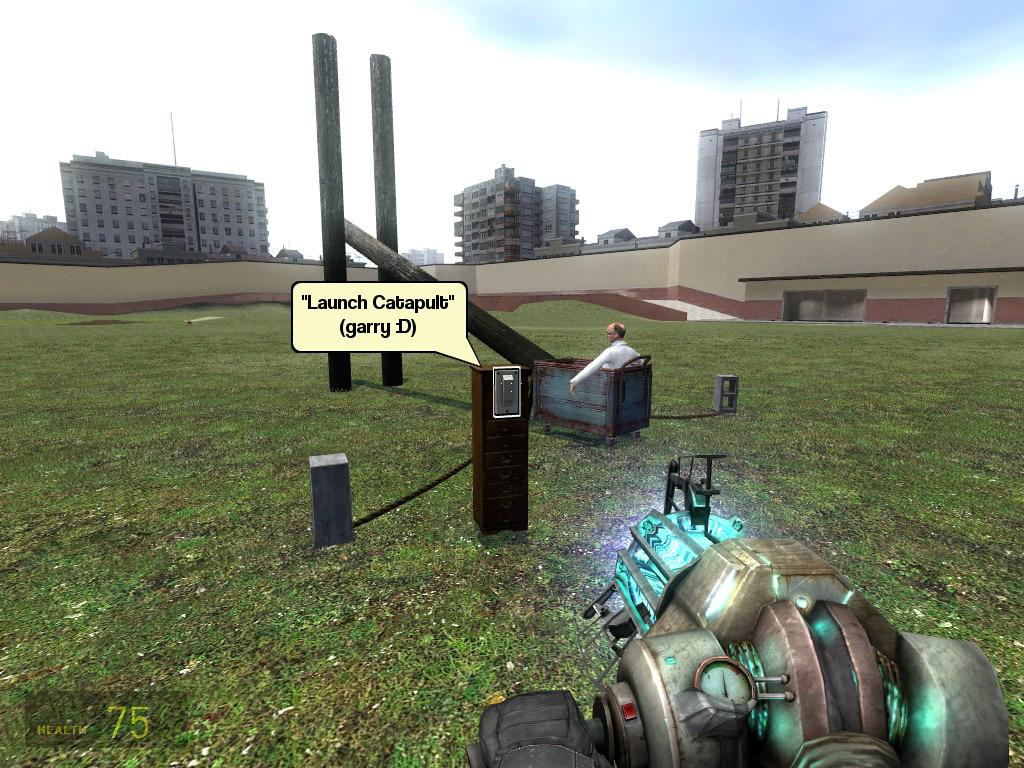
\includegraphics[width=\textwidth]{garrysmod}
\end{frame}

\begin{frame}
\frametitle{Представление моделей}

\begin{itemize}
\item Полигональное \\
Простая, быстрая, экономичная по памяти модель
\item Воксельное \\
Реалистичная модель с возможностью изменения в реальном времени
\end{itemize}
Нужна скорость --- полигональное представление.
\end{frame}

\begin{frame}
\frametitle{Удаление невидимых линий}

\begin{itemize}
\item Алгоритм Робертса \\
Точный, медленный, сложный
\item Алгоритм Вейлера-Азертона \\
Быстр на простых сценах, рекурсивный
\item Z-буферизация \\
Простой, быстрый на современных машинах
\end{itemize}
Выберем Z-буферизацию из-за скорости
\end{frame}

\begin{frame}
\frametitle{Модели освещения}

\begin{itemize}
\item Модель Кука-Торренса \\
Бликовое освещение, точный, медленный
\item Модель Ламберта \\
Простая, описывает диффузное освещение
\item Модель Фонга \\
Эмпирическая, относительно быстрая
\item Модель Блинна-Фонга \\
Точный для разных материалов, медленее чем Фонг
\end{itemize}
Для скорости выбрали модель Фонга
\end{frame}

\begin{frame}
\frametitle{Векторы и матрицы}

\begin{itemize}
\item Храним в массивах
\item Афинные преобразования --- матрицы 3х4 достаточно
\item Реализованы алгоритмы вычисления углов, извлечения эйлеровых координат и.т.д.
\item Перспективное преобразование реализовано отдельно, не матрицей
\end{itemize}
\end{frame}

\begin{frame}
\frametitle{Хранение моделей}
\framesubtitle{Хранение точек}

\begin{itemize}
\item Точки массивом \\
Экономично, быстро, неэффективно если точки меняются
\item Точки списком \\
Медленнее но быстрее добавление/удаление
\item BSP-дерево \\
Специальное дерево, медленно если объект движется
\end{itemize}
Точки не будут меняться --- выберем массив.
\end{frame}

\begin{frame}
\frametitle{Хранение моделей}
\framesubtitle{Многоугольники}

\begin{itemize}
\item Хранить многоугольники --- требуется обрабатывать случаи невыпуклости
\item Треугольники --- однозначно задают плоскость, не требуют проверок
\item В графических библиотеках используются треугольники
\end{itemize}
Выберем треугольники.
\end{frame}

\begin{frame}
\frametitle{Хранение моделей}
\framesubtitle{Хранение треугольников}

\begin{itemize}
\item Хранить как наборы точек \\
Частые повторы.
\item Хранить как наборы индексов в общем массиве точек \\
Значительно экономичнее, чуть медленнее. Используется в графических библиотеках.
\end{itemize}
Будем хранить наборами индексов.
\end{frame}

\begin{frame}
\frametitle{Хранение моделей}
\framesubtitle{Что ещё нужно хранить}

\begin{itemize}
\item Нормали к вершинам --- получаем из файла
\item Нормали к сторонам --- высчитываем векторным произведением.
\item Материал для каждой стороны.
\item UV-координаты.
\end{itemize}
\end{frame}

\begin{frame}
\frametitle{Материал}

\begin{itemize}
\item Храним параметры для освещения
\item Возможно, текстуру
\end{itemize}
\end{frame}

\begin{frame}
\frametitle{Объект на сцене}
\framesubtitle{Структура данных}

\begin{itemize}
\item Храним ссылку на модель
\item Положение объектов на экране
\item Кэшированные преобразованные точки
\item Оверлей материалов
\end{itemize}
\end{frame}

\begin{frame}
\frametitle{Объект на сцене}
\framesubtitle{Позиция}

\begin{itemize}
\item Хранить матрицей \\
Неудобно для редактирования пользователем
\item Хранить эйлеровыми углами и начальной точкой \\
Не всегда удобно для преобразований, но удобно для пользователя.
\end{itemize}
Выберем второй вариант --- пользователь сможет удобно задавать позиции.
\end{frame}

\begin{frame}
\frametitle{Объект на сцене}
\framesubtitle{Источник света}

\begin{itemize}
\item Объект может быть источником света
\item В таком случае хранит параметры для модели освещения
\end{itemize}
\end{frame}

\begin{frame}
\frametitle{Объект на сцене}
\framesubtitle{Кэш}

\begin{itemize}
\item Объект задаётся моделью и позицией
\item Каждый раз преобразовывать точки модели в мировую СК --- медленно
\item Позиция объекта меняется не так часто
\item Будем хранить результаты преобразований
\end{itemize}
\end{frame}

\begin{frame}
\frametitle{Объект на сцене}
\framesubtitle{Оверлей материалов}

\begin{itemize}
\item Хотим заменить у конкретного объекта материал конкретной стороны
\item Будем хранить словарь ``номер вершины --- новый материал''
\item Словарь пополняется со стороны
\end{itemize}
\end{frame}

\begin{frame}
\frametitle{Сцена}

\begin{itemize}
\item Поскольку не используем BSP-дерево, храним просто множество объектов
\item Массив \\
Медленный для изменения количества
\item Связный список \\
Медленнее массива, но быстрое добавление/удаление
\end{itemize}
Предполагается добавление/удаление объектов --- будем использовать связный список.
\end{frame}

\begin{frame}
\frametitle{Отрисовка}
\framesubtitle{Камера}

\begin{itemize}
\item Храним камеру также как позицию объекта
\item Переводим точки в её систему координат
\end{itemize}
\end{frame}

\begin{frame}
\frametitle{Отрисовка}
\framesubtitle{Источники света}

\begin{itemize}
\item Каждый объект может быть источником света
\item Перед преобразованиями создаётся массив параметров источников
\end{itemize}
\end{frame}

\begin{frame}
\frametitle{Отрисовка}
\framesubtitle{Кэш точек}

\begin{itemize}
\item Необходимо хранить преобразованные точки
\item Выделять память каждый кадр --- маедленно
\item Будем хранить между кадрами аллоцированную память для точек и пр.
\end{itemize}
\end{frame}

\begin{frame}
\frametitle{Отрисовка}
\framesubtitle{Отсечение по направлению грани}

\begin{itemize}
\item Часть выпуклого объекта всегда заслонена от наблюдателя
\item Можно не отрисовывать то, что не может быть видимо
\item Определяем по направлению нормали к грани и направлению камеры
\end{itemize}
\end{frame}

\begin{frame}
\frametitle{Отрисовка}
\framesubtitle{Отсечение по плоскостям}

\begin{itemize}
\item Использовать высчитанную нормаль к грани \\
Не учитывает перспективное преобразование, будут артефакты.
\item Высчитывать нормаль после преобразований \\
Учитывает перспективу
\end{itemize}
Используем второй вариант, но реализовываем оба для сравнения скорости.
\end{frame}







\begin{frame}
\frametitle{Структуры данных}
\framesubtitle{Модель}

\begin{itemize}
\item Массив точек --- X, Y, Z, W
\item Массив треугольников --- три индекса точек
\item Массив нормалей для вершин и треугольников
\item Материалы для каждого треугольника
\item Материалы --- цвет или текстура
\item UV-координаты для каждой точки
\end{itemize}
\end{frame}

\begin{frame}
\frametitle{Структуры данных}
\framesubtitle{Объект на сцене}

\begin{itemize}
\item Указатель на модель
\item Позиция --- X, Y, Z, углы разворота
\item Словарь замены материалов --- нужен для изменения материала для объекта
\item Преобразованные относительно позиции точки и нормали модели
\end{itemize}
\end{frame}

\begin{frame}
\frametitle{Растеризация}
\framesubtitle{Последовательность действий}

\begin{itemize}
\item Отсечение треугольников по нормалям
\item Преобразование точек в систему координат камеры, перспективное \item преобразование
\item Отсечение треугольников по плоскостям
\item Обход треугольников по САР
\item Отсечение невидимых граней --- Z-буфер
\item Билинейная интерполяция для текстур
\item Закраски
\end{itemize}
\end{frame}

\begin{frame}
\frametitle{Растеризация}
\framesubtitle{Отсечение по нормалям}

\begin{itemize}
\item Без отсечения --- медленно
\item Грубое отсечение --- быстро, с артефактами
\item Отсечение с учётом перспективы
\end{itemize}
\end{frame}

\begin{frame}
\frametitle{Растеризация}
\framesubtitle{Закраски}

\begin{itemize}
\item Без учёта освещения
\item Плоская закраска --- освещение для каждой грани
\item Закраска по Гуро --- отсечение для каждой вершины
\item Закраска по Фонгу --- отсечение для каждой точки
\end{itemize}
\end{frame}

\begin{frame}
\frametitle{Загрузка моделей}

\begin{itemize}
\item Модели хранятся и загружаются в формате DirectX .x, поддерживается полная спецификация формата
\item Список доступных моделей хранится в формате YAML
\item Для модели хранится название
\end{itemize}
\end{frame}

\begin{frame}
\frametitle{Загрузка и сохранение сцены}

\begin{itemize}
\item Сцена загружается и сохраняется в YAML-файл
\item Хранится список объектов:
  \begin{itemize}
  \item Название модели объекта
  \item Позиция объекта
  \end{itemize}
\end{itemize}
\end{frame}

\begin{frame}
\frametitle{Редактирование сцены}

\begin{itemize}
\item Перемещение, поворот объектов
\item Добавление, удаление объектов из списка доступных моделей
\item Есть привязки к плоскостям других моделей
\end{itemize}
\end{frame}

\begin{frame}
\frametitle{Проблемы и их решения}

Реальное время, нужно много оптимизаций для приемлемой скорости (поставлена цель в 60 кадров в секунду в большинстве случаев)
\begin{itemize}
\item Эффективные структуры данных
\item Оптимизация работы с памятью
\item Хранение полезных промежуточных вычислений
\item Локальные оптимизации
\item Итог --- 60 кадров в секунду при включённых оптимизациях компилятора на всех тестовых сценах, вплоть до 1000 на простых сценах (куб)
\end{itemize}
\end{frame}

\begin{frame}
\frametitle{Проблемы и их решения}

При этом нужно сохранять красивую архитектуру программы
\begin{itemize}
\item Разделённый по этапам конвейер
\item Слои, поддержка элементов управления, обработчиков событий
\item Максимальное разделение функциональности
\item Масштабируемость
\end{itemize}
\end{frame}

\begin{frame}
\frametitle{Проблемы и их решения}

Наличие только базового функционала
\begin{itemize}
\item Проект на C++/SDL — очень быстро но мало встроенных возможностей
\item Реализованы стандартные алгоритмы отрисовки линий и закраски
\item Реализованы элементы управления --- текстовые, списки с выбором, строки ввода
\end{itemize}
\end{frame}

\begin{frame}
\frametitle{Проблемы и их решения}

Загрузка и сохранение в файлы
\begin{itemize}
\item Написан парсер, поддерживающий почти полную спецификацию DirectX .x (с использованием lexx и bison)
\item Использование стороннего парсера для YAML
\item Настройки программы тоже в отдельном YAML-файле
\end{itemize}
\end{frame}

\begin{frame}
\frametitle{Внешний вид}

\centering
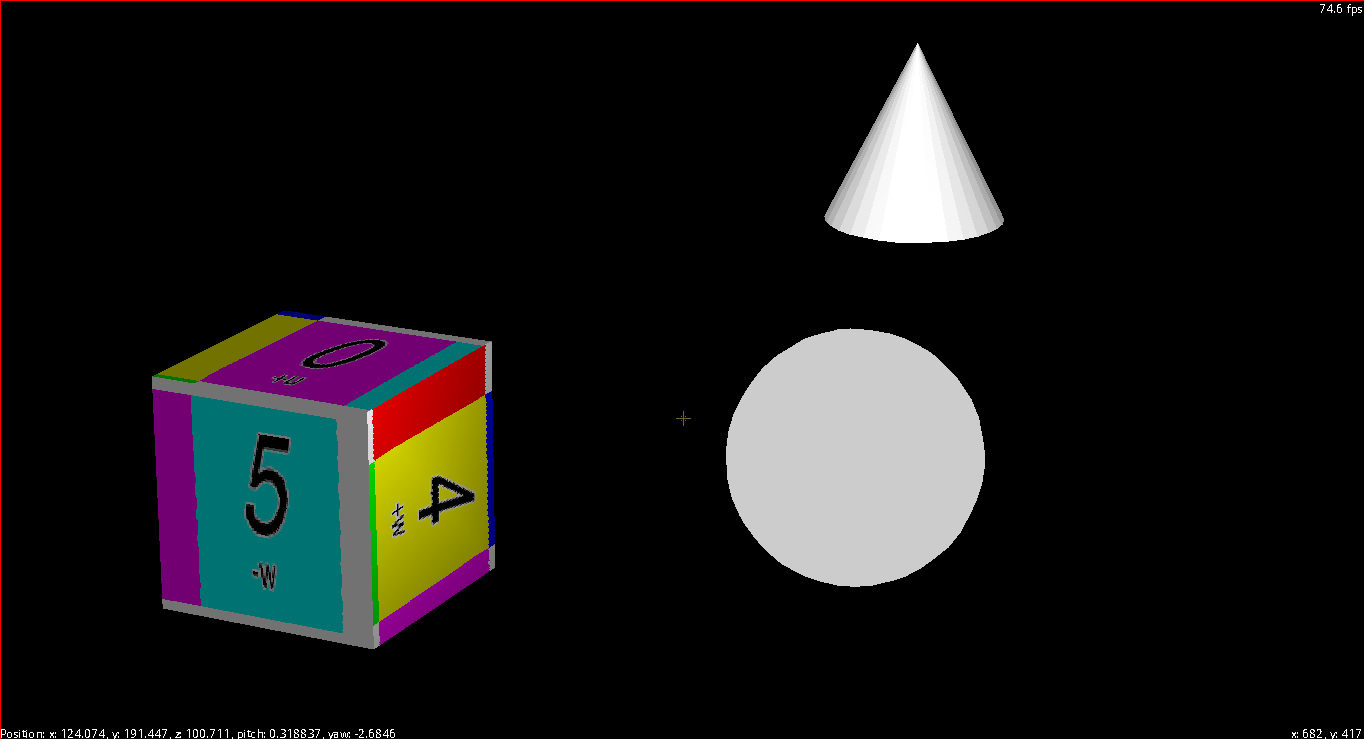
\includegraphics[width=\textwidth]{window}
\end{frame}

\begin{frame}
\centering
Спасибо за внимание!
\end{frame}

\end{document}